% !TEX encoding = UTF-8
% !TEX TS-program = pdflatex
% !TEX root = computabilità e algoritmi.tex
% !TEX spellcheck = it-IT

\subsection{L'algoritmo bit a bit}

Assumiamo che la nostra rete sia un ipercubo, ovvero, rappresentando in bit il numero del nodo, c'è un canale tra due nodi solo se i due nodi differiscono di un bit. Il collegamento può essere considerato bi-direzionale.

Un ipercubo di dimensione $k$ ha $n=2^k$ vertici numerati da 0 a $n-1$ e ogni vertice è etichettato con la rappresentazione binaria $i_0 \ldots i_{k-1}$ del suo numero d'ordine.
I canali di comunicazione sono $kn$, dato che ogni processore ha $k$ canali di input e $k$ canali di output.

Due processori sono connessi se le loro due rappresentazioni binarie differiscono di un solo bit.

L'algoritmo \textbf{bit a bit} consiste nel fissare un bit della destinazione alla volta: l'algoritmo confronta i bit della destinazione con i bit del processore in cui si trova attualmente il pacchetto e lo invia sul canale corrispondente al primo bit diverso.

Questo algoritmo è \textbf{ignaro} in quanto calcola il percorso del pacchetto prendendo in considerazione solamente il processore di partenza e quello di arrivo, senza considerare il percorso degli altri pacchetti.

Ad esempio, assumendo di avere $k=4$ e di dover mandare un pacchetto da $i = 1011$ a $d_i = 1100$. Per trovare un cammino si deve cercare di rendere simili i codici binari, ovvero si passa prima per $1111$ e $1101$, per arrivare in fine a $1100$.

\subsection{Algoritmo randomizzato}\label{una-prima-versione-dellalgoritmo-randomizzato}

Per ciascuno degli \emph{n} processori sceglie una destinazione intermedia $\sigma_i$ in modo casuale e indipendente.

Usa l'algoritmo deterministico bit a bit per instradare ogni pacchetto $p_i$ dal processore \emph{i} al processore $\sigma_i$ e poi usa lo
stesso algoritmo per far transitare il pacchetto da $\sigma_i$ a $d_i$.

Nelle code di attesa viene data la precedenza ai pacchetti che devono ancora arrivare alla destinazione intermedia.

Per gestire la coda dei canali di comunicazione si ha che i pacchetti della prima fase, quelli che vanno dalla sorgente alla tappa intermedia hanno la priorità su quelli che vanno dalla fase intermedia alla destinazione.

Consideriamo solamente il tempo necessario per la prima fase: la durata è data dal numero \emph{m} di bit diversi che ci sono tra la sorgente e la destinazione intermedia, più il numero di passi in cui il pacchetto rimane in coda. 
Un altro pacchetto può far ritardare il nostro pacchetto di interesse se ha almeno un canale di comunicazione in comune.

(\textbf{Lemma 4.2}) Consideriamo i due pacchetti $p_i$ e $p_j$, che partono rispettivamente da \emph{i} e \emph{j}, cercando di arrivare a $\sigma_i$ e $\sigma_j$.
Sia $s$ l'ultima posizione in cui le due rappresentazioni binarie di $i$ e $j$ differiscono e $t$ la prima posizione in cui differiscono $\sigma_i$ e $\sigma_j$.

\begin{figure}[htbp]
	\centering
	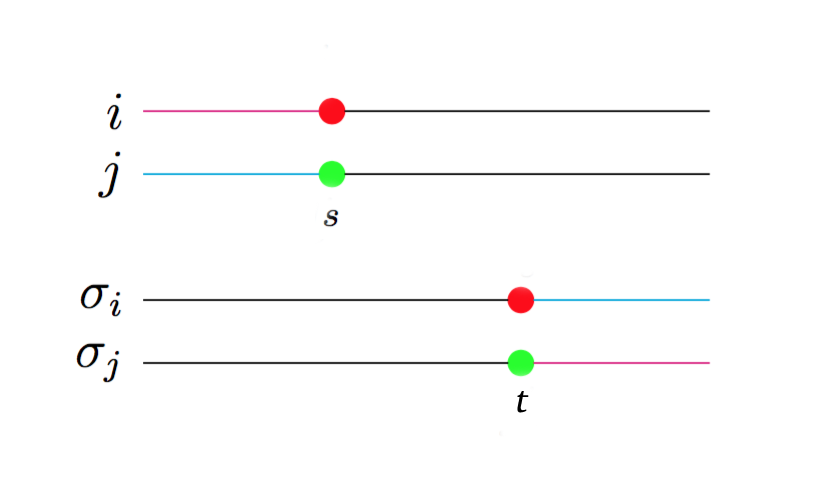
\includegraphics[width=0.4\textwidth]{./notes/immagini/l38-fig1.png}
	\caption{Illustrazione del lemma 4.2. In nero sono disegnate le parti uguali delle rappresentazioni binarie. I bit indicati con il pallino sono diversi, mentre i restanti colorati in azzurro e viola possono essere sia uguali che diversi.}
\end{figure}

Se $s \geq t$ i due percorsi non hanno processori in comune e quindi non si incrociano mai.

Se $s  < t$ i due pacchetti stanno su processori distinti finché l'algoritmo non processa tutti i bit da $0$ a $s$, mentre transitano sugli stessi processori quando vengono processati i bit da $s+1$ a $t-1$, per poi finire su processori diversi dal bit $t$ in poi.

Si ha quindi che il numero di processori in comune è dato da $t - s - 1$ e i canali in comune sono quindi $t-s-2$ e sono anche consecutivi tra loro.

Supponiamo che $p_i$ segua il percorso $\rho_i = e_1, e_2, \ldots, e_m$ con $m \leq k$. 
Questo pacchetto può essere rallentato solamente da un pacchetto che ha un canale in comune.

Per valutare i ritardi, l'idea è quella di attribuire la causa di un'unità di tempo di ritardo ad ogni pacchetto, ovvero di andare a maggiorare il ritardo considerando i pacchetti che hanno almeno un canale in comune.

Supponiamo che il nostro pacchetto \emph{i} transiti per:

$$
i \bullet \rightarrow e_1 \bullet\rightarrow e_2\bullet \rightarrow \ldots \rightarrow e_{h-1} \bullet \rightarrow e_h \bullet \rightarrow \ldots \rightarrow e_{m}\bullet
$$

e che all'istante \emph{t} il pacchetto si trovi in coda nel nodo tra $e_{h-1}$ e $e_h$.

Ovvero c'è un pacchetto $p(t,h)$ che transita sul canale \emph{h} mentre il nostro pacchetto è in coda.

All'istante $t+1$, il pacchetto rompi scatole si troverà nel processore successivo. 
Può quindi essere arrivato a destinazione, proseguire su un canale diverso da quello che interessa a noi oppure proseguire sul nostro cammino.

In ogni caso, il pacchetto rompi scatole non creerà più ritardi al nostro pacchetto, perché quando percorre $e_{h+1}$ il nostro pacchetto o è ancora in coda o è in $e_h$. 

Se il pacchetto rompi scatole resta invece fermo in coda e deve proseguire sulla nostra strada, vuol dire che all'istante $t+2$ c'è un'altro pacchetto $p(t+1, h+1)$ che è passato sul canale al posto suo. 
In questo caso si può associare il ritardo del nostro pacchetto a $p(t+1, h+1)$.

La storia si ripete anche per gli istanti successivi, ma prima o poi si arriverà ad una fine, perché il cammino è lungo \emph{k}.

Da questo deriva il \textbf{Lemma 4.3}: Sia $\rho_i = e_1, e_2 \ldots e_m$ il percorso di un pacchetto $p_i$ e supponiamo che al tempo $t$ esso abbia attraversati i primi $h$ canali del suo cammino e si trovi nella coda del canale $e_{h+1}$ con un ritardo accumulato di $l = t-h$. Se il pacchetto $p_i$ nel passo successivo rimane bloccato nella coda allora, per qualche $k\geq 1$ deve esistere un altro pacchetto $p$ che dopo aver percorso l'arco $e_{h+k}$ del cammino $p_i$ al tempo $t+k = h+k+l$, al tempo $t+kè1$ esce dal cammino $\rho_i$ perché arrivato a destinazione oppure perché procede su un canale diverso.

Quindi per ogni ritardo $l = 0, \ldots, r-1$ associo un pacchetto il cui cammino ha almeno un canale in comune con quello di interesse.

Se $p_i$ impiega tempo \emph{t} con un ritardo totale di che è uguale a $r = t -m$, allora devono esserci almeno altri \emph{r} pacchetti con un canale in comune.

Siano due pacchetti $p_i$ e $p_j$ e $X_{ij}$ la variabile aleatoria che vale 1 se i due pacchetti hanno un canale in comune e 0 altrimenti.

Così facendo si ha che il ritardo $r_i$ del pacchetto \emph{i} è dato da

$$
r_i \leq \sum\limits_{j \neq i} X_{i,j} < \sum\limits_{j} X_{i,j} \leq \sum\limits_{i = 1}^{m} P(e_i)
$$

dove $P(e_i)$ è il numero totale di pacchetti che passano per il canale $e_i$.

Si ha quindi che

$$
E[r_i] \leq \sum\limits_{j \neq i} E[X_{i,j}] \leq \sum\limits_{j} E[X_{i,j}] \leq \sum\limits_{i = 1}^{m} E[P(e_i)]
$$

Dal momento che le destinazioni intermedie sono scelte a caso, si ha che il valore atteso di $P(e_i)$ non dipende dal canale, dato che l'ipercubo è perfettamente simmetrico.

Il valore atteso della lunghezza di un cammino generico è $E[m] = k/2$, perché dal momento che la destinazione intermedia viene scelta casualmente, ogni bit ha probabilità 1/2 di essere diverso dal corrispondente bit del processore di partenza. 
Considerando che ci sono $k 2^k$ canali e che il valore atteso della somma dei canali percorsi è $k/2 \cdot  2^{k}$, si ha che il valore atteso dei pacchetti che passano su un canale qualsiasi è $1/2$ e quindi

$$
\sum\limits_{i = 1}^{m} \textbf{E}[P(e_i)] = m/2 \leq k/2
$$

Quindi il ritardo medio di un singolo pacchetto minore o uguale di $k/2$.

Consideriamo la variabile casuale

$$
X = \sum\limits_{j \neq i} X_{i,j}
$$

la probabilità che $X_{i,j}$ sia uguale a 1 è sicuramente minore di 1 e la media $\mu =E[X]$ è minore o uguale di $k/2$ per quanto detto prima.

Sotto queste ipotesi è possibile applicare il limite di Chernov:

$$
Pr[X > (1 + \delta)\frac{k}{2}] \leq \Big[ \frac{e^\delta}{(1+\delta)^{1+\delta}} \big]^{k/2}
$$

Se prediamo $\delta = 7$, abbiamo che

$$
Pr[X > 4k] \leq  [\frac{e^7}{8^8}]^{k/2} < 2^{-6k}
$$

ovvero la probabilità che un pacchetto impieghi più di $4k$ per arrivare a destinazione è minore di $2^{-6k}$.

Siccome i pacchetti sono \emph{n}, la probabilità che almeno uno arrivi dopo $4k$ è minore o uguale di $2^{-5k} = 1/32^k$. Analogamente, la probabilità che tutti i pacchetti arrivino a destinazione con un ritardo inferiore a $4k$ (ovvero in meno di $5k$) è $1-1/32^k$

Tutto questo riguarda la prima fase.

La seconda fase può essere analizzata allo stesso modo della prima fase, la differenza è che nella prima fase i pacchetti partono contemporaneamente mentre nella seconda, se non viene aspettato il termine della prima fase, la partenza della seconda fase avviene in momenti diversi.

In ogni caso, la maggiorazione dei ritardi della prima fase è stata fatta senza tenere conto della partenza dei pacchetti. 
Se le partenze sono diverse non ci sarà un'interferenza ma la maggiorazione continua a valere.

Si può quindi dire che anche nella seconda fase valgono le stesse probabilità.

Tirando le somme, il tempo richiesto dalla prima fase è minore o uguale di $5k$ e anche quello della seconda fase, con probabilità $ 1-1/32^{k}$.
Ovvero i pacchetti saranno tutti a destinazione in tempo $10k$ con probabilità maggiore o uguale di $1- 1/32^k$.

Se ad esempio $k = 32$, si ha tempo 320 con probabilità maggiore o uguale di $1 - 1/32^{32}$, ovvero con una certezza quasi assoluta. 
Mentre Valiant dava un tempo massimo di $11585$, che rappresenta un caso pessimo ma probabile, mentre con questo nuovo algoritmo si ha un caso pessimo poco probabile e che è di gran lunga migliore.
